\documentclass[fleqn,11pt,a4paper,dvipdfmx]{jsarticle}
%
\usepackage{amsmath,amssymb}
\usepackage{bm}
\usepackage[dvipdfmx]{graphicx}
\usepackage{bmpsize}  % ← バウンディングボックス用
\usepackage{ascmac}
\usepackage{multicol} 
\usepackage{paracol}
\usepackage{tikz}
\usepackage{caption}
\usepackage{amsmath}
\usepackage{mathtools}
\captionsetup[table]{justification=centering}
\captionsetup[figure]{justification=centering}
\usetikzlibrary{calc}
\renewcommand{\thefigure}{\thesection.\arabic{figure}}
% \setlength{\textwidth}{\fullwidth}
% \setlength{\textheight}{39\baselineskip}
% \addtolength{\textheight}{\topskip}
% \setlength{\voffset}{-0.5in}
% \setlength{\headsep}{0.3in}
% \setlength{\mathindent}{0pt}  % 数式の左端インデントを0に
\vspace*{-\baselineskip} % ← 不要な最初の空白を詰める
\usepackage[
  left=2cm,    % 左だけ広め
  right=2cm,   % 右は狭め
  top=2cm,     % 上も狭め
  bottom=1.5cm   % 下も狭め
]{geometry}
%
\newcommand{\divergence}{\mathrm{div}\,}  %ダイバージェンス
\newcommand{\grad}{\mathrm{grad}\,}  %グラディエント
\newcommand{\rot}{\mathrm{rot}\,}  %ローテーション

\numberwithin{equation}{section}
\setcounter{equation}{16}

%
% \pagestyle{myheadings}
\begin{document}
%
%
1 AEI 3番 : 馬場 悠斗
\setcounter{section}{12}
\subsection{線形負荷のみの補償に関する方程式}

線形負荷と非線形負荷の並列組み合わせ
図12.1の非線形荷重を取り除いたとする. 
すると, 図12.2では
\begin{equation}
  i_l = 0
\end{equation}

\begin{equation}
  i = i_b = \frac{e_{in}}{\left(Z_a + Z_d\right)}
\end{equation}

添え字'1'は, 基本周波数または電源周波数に対するインピーダンスを示す. 
は, 電流の基本波または電源周波数の高調波に対するインピーダンスを示す. 
合成入力インピーダンスを$Z_a1d1$とする. 
\begin{equation}
  Z_{a1d1} = Z_{a1} + Z_{d1} = |Z_{a1d1}| \angle \Phi_{a1d1}
\end{equation}

ここで
\begin{equation}
  |Z_{a1d1}| = \sqrt{|Z_{a1}|^2 + |Z_{d1}|^2 + 2|Z_{a1}||Z_{d1}| \cos \left(\Phi_{a1} - \Phi_{d1}\right) }
\end{equation}
である
\begin{equation}
  \Phi_{a1d1} = \tan^{-1}\left( \frac{\left| Z_{a1} \right| \sin \Phi_{a1} + \left| Z_{d1} \right| \sin \Phi_{d1} }{\left| Z_{a1} \right| \cos \Phi_{a1} + \left| Z_{d1} \right| \cos \Phi_{d1}}\right)
\end{equation}

ここで, コンデンサ$Z_c$(図12.2)を取り除くとします. 
この条件では
\begin{equation}
  Z_{d1} = Z_{b1}
\end{equation}
(12.8)を(12.22)に組み合わせると
\begin{align}
  i & = \frac{e_{in}}{\left| Z_{a1d1}\angle Z_{a1d1} \right|} = i_b \notag                     \\
    & = \sqrt{2} \frac{E_{in}}{\left|Z_{a1d1}\right|} \sin \left(\omega t - \Phi_{a1d1}\right)
\end{align}

\setcounter{figure}{1}
\begin{figure}[b]
  \begin{center}
    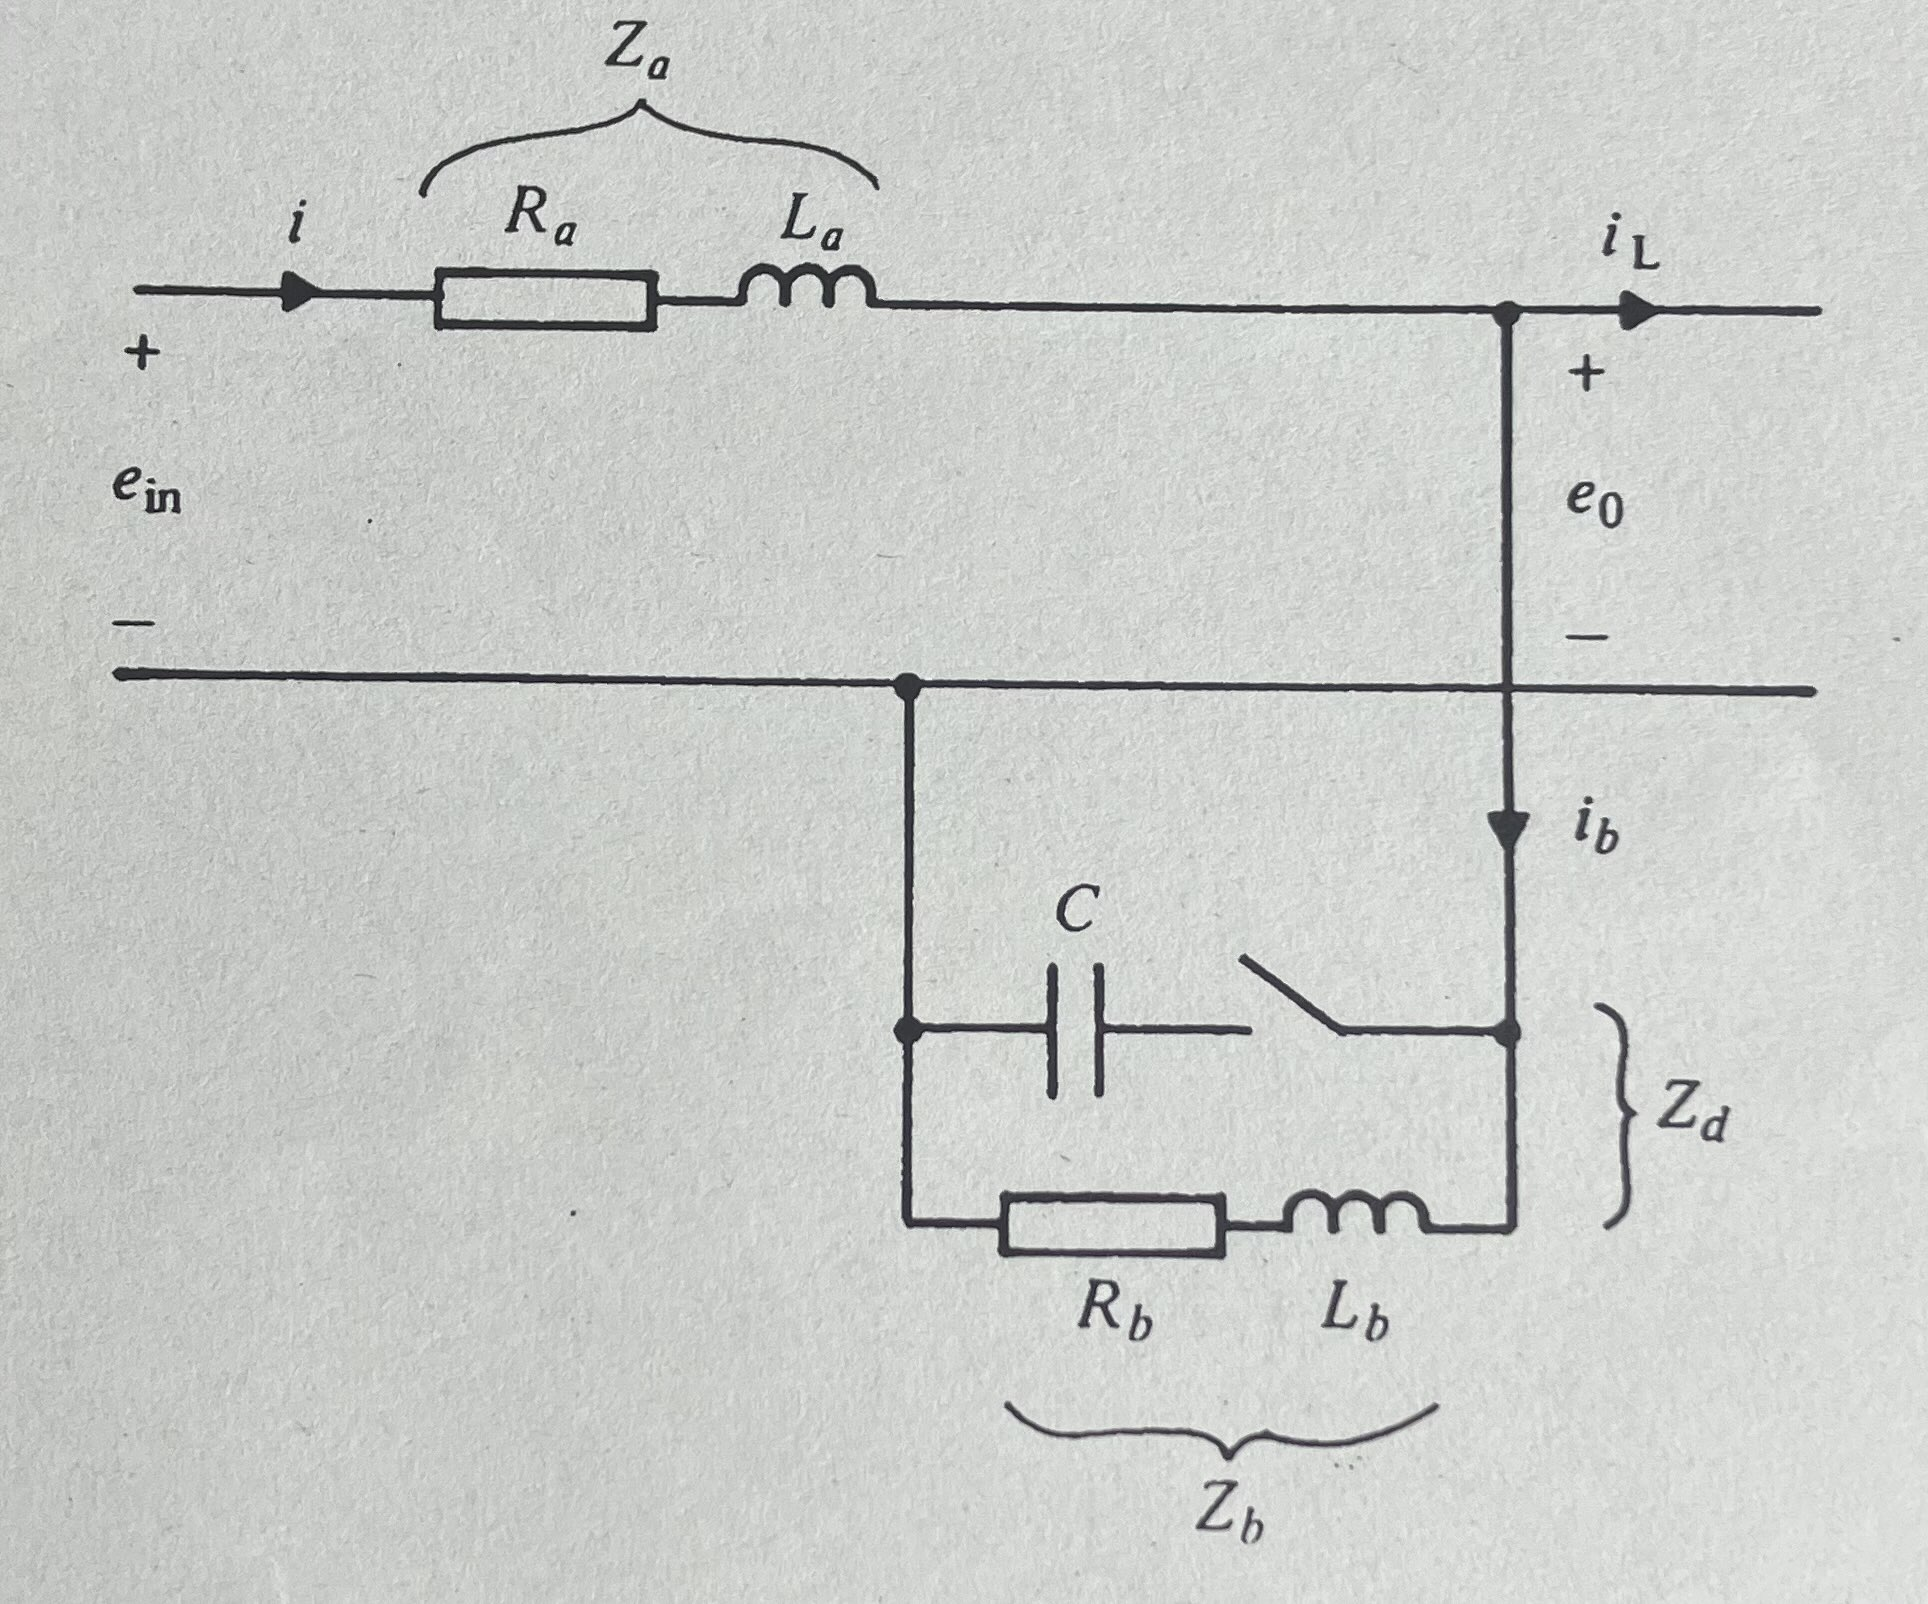
\includegraphics[width=100mm]{./img/circuit.jpg}
    \caption{図12.1において線形部分の等価回路}
    \label{circuit}
  \end{center}
\end{figure}

\newpage

線形, 非補償負荷$Z_b$に対する条件では, 負荷電圧$e_0$は次のように修正されます. 

\begin{equation}
  e_0 = i_b \left(\left|Z_{b1} \angle \Phi_{b1}\right|\right)
\end{equation}

(12.23)と(12.24)を組み合わせると

\begin{equation}
  e_0 = \sqrt{2} \frac{E_{in}}{\left|Z_{a1d1}\right|} \left|Z_{b1}\right| \sin \left(\omega t - \Phi_{a1b1} + \Phi_{b1}\right)
\end{equation}

負荷における電流$i$ は, 純粋な抵抗と純粋なリアクタンスの等価並列負荷が使用された場合に流れる仮想成分$i_R$,$i_x$($e_0$に関して)に分解できる. 

\begin{equation}
  i_R = \sqrt{2} \frac{E_{in}}{\left|Z_{a1b1}\right|} \cos \Phi_{b1} \sin \left(\omega t - \phi_{a1b1} + \Phi_{b1}\right)
\end{equation}

\begin{equation}
  i_X = \sqrt{2} \frac{E_{in}}{\left|Z_{a1b1}\right|} \sin \Phi_{b1} \sin \left(\omega t - \Phi_{a1b1} + \Phi_{b1}\right)
\end{equation}

(12.26)および(12.27)の実効形式を(12.25)の実効形式と組み合わせると, 負荷端子における皮相電力の成分が得られる. 

\begin{equation}
  S_R = \frac{{E_{in}}^2 \left|Z_{b1}\right|}{{\left|Z_{a1b1}\right|}^2}\cos\Phi_{b1}
\end{equation}

\begin{equation}
  S_X = \frac{{E_{in}}^2 \left|Z_{b1}\right|}{{\left|Z_{a1b1}\right|}^2}\sin\Phi_{b1}
\end{equation}

負荷での力率一定値動作では, コンデンサC, 
は, (12.27)の$i_x$を補償し, それによって(12.29)の$S_x$に等しい定格電圧を持たなければならない. 

\begin{equation}
  \left|Z_C\right| = \frac{\left|Z_{b1}\right|}{\sin \Phi_{b1}}
\end{equation}

\begin{equation}
  C = \frac{\sin \Phi_{b1}}{\omega \left|Z_{b1}\right|}
\end{equation}

補償された負荷の端子を見たインピーダンス$Z_{d1}$ は, 次式で与えられる. 

\begin{equation}
  Z_{d1} = \frac{\left|Z_{b1}\right|}{\cos \Phi_{b1}} \angle 0
\end{equation}

完全に補償された負荷の場合, 入力インピーダンス(12.32)は純粋な抵抗性である. 


\newpage
words

\newpage
\setcounter{section}{1}
\setcounter{figure}{0}
\section*{式の導出}
\subsection*{式(12.20)の導出}
\begin{figure}[b]
  \begin{center}
    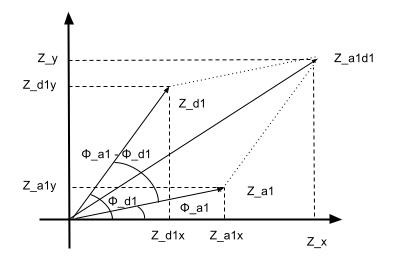
\includegraphics[width=100mm]{./img/vector_Z.jpg}
    \caption{ベクトルのイメージ図}
    \label{vector_Z}
  \end{center}
\end{figure}


各インピーダンスの成分をそれぞれ
$Z_{a1} = \left(Z_{a1x} , Z_{a1y}\right) , Z_{d1} = \left(Z_{d1x} , Z_{d1y}\right) $
とすると, 合成インピーダンス$Z_{a1d1}$の成分は$Z_{a1d1} = \left(Z_x , Z_y\right)$は, 
$Z_x = Z_{a1x} + Z_{d1x} , Z_y = Z_{a1y} + Z_{d1y}$となる. これらの関係を図\ref{vector_Z}に示す. \\
$Z_{a1d1}$の大きさは,\\
\begin{align*}
  \left|Z_{a1d1}\right| & = \sqrt{ {\left(Z_x\right)}^2 + {\left(Z_y\right)}^2 }                                                                                            \\
                        & = \sqrt{ {\left(Z_{a1x} + Z_{d1x}\right)}^2 + {\left(Z_{a1x} + Z_{d1x}\right)}^2 }                                                                \\
                        & = \sqrt{ \left( {Z_{a1x}}^2 + 2Z_{a1x}Z_{d1x} + {Z_{d1x}}^2 \right) + \left( {Z_{a1y}}^2 + 2Z_{a1y}Z_{d1y} + {Z_{d1y}}^2 \right)}                 \\
                        & =  \sqrt{ \left( {Z_{a1x}}^2 + {Z_{a1y}}^2 + {Z_{d1x}}^2  + {Z_{d1y}}^2 \right) + \left(2Z_{a1x}Z_{d1x} + 2Z_{a1y}Z_{d1y}  \right)}               \\
                        & =  \sqrt{ \left( {Z_{a1x}}^2 + {Z_{a1y}}^2 \right) + \left({Z_{d1x}}^2  + {Z_{d1y}}^2 \right) + \left(2Z_{a1x}Z_{d1x} + 2Z_{a1y}Z_{d1y}  \right)} \\
                        & =  \sqrt{ \left( {Z_{a1x}}^2 + {Z_{a1y}}^2 \right) + \left({Z_{d1x}}^2  + {Z_{d1y}}^2 \right) + 2\left(Z_{a1x}Z_{d1x} + Z_{a1y}Z_{d1y}  \right)}  \\
\end{align*}
$\left|Z_{a1}\right| = \sqrt{{{Z_{a1x}}^2 + {Z_{a1y}}^2}},\left|Z_{d1}\right| = \sqrt{{{Z_{d1x}}^2 + {Z_{d1y}}^2}}$である. \\
また, 各インピーダンスをベクトルと考え, この2つのベクトルの成す角を$\Phi_{a1} - \Phi_{d1}$とすると, \\
$\left(Z_a , Z_d\right) = Z_{a1x}Z_{d1x} + Z_{a1y}Z_{d1y} = \left|Z_{a1}\right| \left|Z_{d1}\right| \cos \left(\Phi_{a1} - \Phi_{d1}\right)$であるから, 
これらを代入すると, 
\begin{equation*}
  \left|Z_{a1d1}\right| = \sqrt{ {\left|Z_{a1}\right|}^2 + {\left|Z_{d1}\right|}^2 + 2 \left|Z_{a1}\right| \left|Z_{d1}\right| \cos \left(\Phi_{a1} - \Phi_{d1}\right)}
\end{equation*}
となり, (12.20)が得られる. 

\newpage
\subsection*{式(12.21)の導出}
まず, tanの定義より, $\tan\left(\Phi_{a1} - \Phi_{d1}\right) = \frac{Z_y}{Z_x}$であるから, 
逆三角関数を用いて, 
$\left(\Phi_{a1} - \Phi_{d1}\right) = \tan^{-1}\frac{Z_y}{Z_x}$.\\
$Z_{a1d1}$の各成分は
$Z_x = Z_{a1x} + Z_{d1x}$ , $Z_y = Z_{a1y} + Z_{d1y}$ .\\
$Z_{a1}$,$Z_{d1}$のx,y成分はそれぞれ\\
$Z_{a1x} = \left|Z_a\right| \cos \Phi_{a1}$ ,$Z_{a1y} = \left|Z_a\right| \sin \Phi_{a1}$\\
$Z_{d1x} = \left|Z_d\right| \cos \Phi_{d1}$ ,$Z_{d1y} = \left|Z_d\right| \sin \Phi_{d1}$\\
であるから, 
\begin{align*}
  \Phi_{a1d1} = \tan^{-1}\left( \frac{\left| Z_{a1} \right| \sin \Phi_{a1} + \left| Z_{d1} \right| \sin \Phi_{d1} }{\left| Z_{a1} \right| \cos \Phi_{a1} + \left| Z_{d1} \right| \cos \Phi_{d1}}\right)
\end{align*}
が得られる. 

\subsection*{式(12.23)の導出}
% まず, 式(12.8)は, 
% \begin{equation*}
%   i_{bx} = \sqrt{2} \sum_{1}^{n} \frac{E_n}{\left|Z_{dn}\right|} \sin \Phi_{dn} \cos \left(n\omega t + \alpha_n\right)
% \end{equation*}
まず, 式(12.18)は, 
\begin{equation*}
  i = i_b = \frac{e_{in}}{\left(Z_a + Z_d\right)}
\end{equation*}
図12.2からキャパシタを除去した場合, $Z_d$部分は,$Z_b$のみとなり, 
並列部分がなくなるため$i = i_b$が成立する. 
これを式(12.18)に代入すると, 電流$i$は, 
$e_{in} = \sqrt{2}E_{in}\sin \omega t$
であるから, オームの法則を用いて, 
\begin{align*}
  i & = i_b = \frac{e_{in}}{Z_{a1d1}} = \frac{e_{in}}{Z_{a1b1}} = \frac{\sqrt{2}E_{in}\sin \left(\omega t\right)}{\left|Z_{a1b1}\right| \angle \Phi_{a1b1}}
  = \frac{ \sqrt{2}{E_{in}} \angle \left( \omega t \right)}{\left| Z_{a1b1} \right| \angle \Phi_{a1b1}} = \sqrt{2} {\left(\frac{E_{in}}{\left|Z_{a1b1}\right|}\right)} \angle{\left(\omega t - \Phi_{a1b1}\right)} \\
    & = \sqrt{2} \frac{ E_{in} }{\left| Z_{a1b1} \right|}\sin \left(\omega t - \Phi_{a1b1}\right) \\
    \because  z_1 &= \left| z_1 \right| \angle \theta_1 = \left| z_1 \right| \left(\cos \theta_1 + j \sin \theta_1\right) \\
              z_2 &= \left| z_2 \right| \angle \theta_2 = \left| z_2\right| \left(\cos \theta_2 + j \sin \theta_2\right)  \\
              z_1z_2 &= \left| z_1 \right|\left| z_2 \right| \angle \left(\theta_1 + \theta_2\right) = \left| z_1 \right|\left| z_2\right| \left(\cos \left(\theta_1 + \theta_2\right) + j \sin \left(\theta_1 + \theta_2\right)\right)
\end{align*}

が得られる. 

\subsection*{式(12.25)の導出}
式(12.23)及び, (12.24)から, 
\begin{equation*}
  \left\{ \,
  \begin{aligned}
     & i = i_b = \sqrt{2} \frac{ E_{in} }{\left| Z_{a1b1} \right|}\sin \left(\omega t - \Phi_{a1b1}\right) & \left(12.23\right) \\
     & e_0 = i_b \left(\left|Z_{b1} \angle \Phi_{b1}\right|\right)                                         & \left(12.24\right)
  \end{aligned}
  \right.
\end{equation*}
であるから, 
\begin{align*}
  e_0 & = \sqrt{2} \frac{ E_{in} }{\left| Z_{a1b1} \right|}\sin \left(\omega t - \Phi_{a1b1}\right) \cdot \left(\left|Z_{b1}\right| \angle \Phi_{b1}\right) 
  = \sqrt{2} \frac{ E_{in} }{\left| Z_{a1b1} \right|} \left|Z_{b1}\right| \sin {\left(\omega t - \Phi_{a1b1} + \Phi_{b1}\right)}
\end{align*}
が得られる. 

\subsection*{式(12.26),式(12.27)の導出}
式(12.23)から
\begin{align*}
  i = i_b = \sqrt{2} \frac{ E_{in} }{\left| Z_{a1b1} \right|}\sin \left(\omega t - \Phi_{a1b1}\right) & \left(12.23\right) \\
\end{align*}
$Z_b$における電流の抵抗成分とリアクタンス成分に分解するためには、$\cos \Phi_{b1}$成分と$\sin\Phi_{b1}$成分に分解すればよいので、
\begin{equation*}
  \left\{ \,
  \begin{aligned}
  i_R &= i_b \cdot \cos \Phi_{b1} = \sqrt{2} \frac{ E_{in} }{\left| Z_{a1b1} \right|} \cos \Phi_{b1} \sin \left(\omega t - \Phi_{a1b1}\right)\\
  i_X &= i_b \cdot \sin \Phi_{b1} = \sqrt{2} \frac{ E_{in} }{\left| Z_{a1b1} \right|} \sin \Phi_{b1} \sin \left(\omega t - \Phi_{a1b1}\right)
  \end{aligned}  
  \right .
\end{equation*}
が得られる。
\[
  \left(
    \begin{tabular}{l}
      $e_0 = \sqrt{2} \frac{ E_{in} }{\left| Z_{a1b1} \right|} \left|Z_{b1}\right| \sin {\left(\omega t - \Phi_{a1b1} + \Phi_{b1}\right)}$\\ \\
      から、$\left|Z_{b1}\right| \angle \Phi_{b1}$を用いて\\ \\
      $i_R = \frac{e_0}{\left|Z_{b1}\right| \angle \Phi_{b1}} \cdot \cos \Phi_{b1} = \sqrt{2} \frac{ E_{in} }{\left| Z_{a1b1} \right|} \cos \Phi_{b1} \sin {\left(\omega t - \Phi_{a1b1}\right)}$\\ \\
      $i_X = \frac{e_0}{\left|Z_{b1}\right| \angle \Phi_{b1}} \cdot \sin \Phi_{b1} = \sqrt{2} \frac{ E_{in} }{\left| Z_{a1b1} \right|} \sin \Phi_{b1} \sin {\left(\omega t - \Phi_{a1b1}\right)}$\\ \\
      導出しても同様になる。
    \end{tabular}
  \right)
\]


\subsection*{式(12.28),式(12.29)の導出}
皮相電力は、電流と電圧の積であるから、抵抗とリアクタンスのそれぞれの皮相電力は、
\begin{align*}
  ei_R  &= e_0 i_R = \sqrt{2} \frac{ E_{in} }{\left| Z_{a1b1} \right|} \left|Z_{b1}\right|  \sin \left(\omega t - \Phi_{a1b1}\right) \cdot \sqrt{2} \frac{ E_{in} }{\left| Z_{a1b1} \right|} \cos \Phi_{b1} \sin \left(\omega t - \Phi_{a1b1}\right) \\
        &= 2 \frac{{E_{in}}^2}{{\left|Z_{a1b1}\right|}^2}\left|Z_{b1}\right| \cos \Phi_{b1} {\left(\sin \left( \omega t - \Phi_{a1b1}\right)\right)}^2 \\
  ei_X  &= e_0 i_X = \sqrt{2} \frac{ E_{in} }{\left| Z_{a1b1} \right|} \left|Z_{b1}\right| \sin \left(\omega t - \Phi_{a1b1}\right) \cdot \sqrt{2} \frac{ E_{in} }{\left| Z_{a1b1} \right|} \sin \Phi_{b1} \sin \left(\omega t - \Phi_{a1b1}\right) \\
        &= 2 \frac{{E_{in}}^2}{{\left|Z_{a1b1}\right|}^2} \left|Z_{b1}\right| \sin \Phi_{b1} {\left(\sin \left( \omega t - \Phi_{a1b1}\right)\right)}^2 \\
\end{align*}
本文中から、実行形式(rms form)とあるので、実効値の定義から2乗平均の平方根を考える。\\
電圧$e_0$、電流$i_b$に関しては、式(12.1)、式(12.4)からすでに実効値である。
$\cos \Phi_{b1}$及び、$\sin \Phi_{b1}$に関しては定数であるため実効値を考慮しなくて良い。
つまり、${\left(\sin \left( \omega t - \Phi_{a1b1}\right)\right)}^2$の項の実効値を考えればよい。
$\left(\sin \left( \omega t - \Phi_{a1b1}\right)\right)$の実効値は、
\begin{align*}
    & \sqrt{\frac{1}{T} \int_{0}^{T}  \sin^2 \left( \omega t - \Phi_{a1b1}\right)} dt               &\text{(半角の公式)}\\
  = & \sqrt{ \frac{1}{2T} \int_{0}^{T}  1 - \cos 2 \left( \omega t - \Phi_{a1b1}\right)} dt         \\
  = & \sqrt{ \frac{1}{2T} \left[  1 - \sin 2 \left( \omega t - \Phi_{a1b1}\right) \right]_{0}^{T}}  \\
  = & \sqrt{ \frac{1}{2T} \left\{ \left(T - \frac{1}{2\omega} \sin 2 \left( \omega T - \Phi_{a1b1}\right)\right) - 
  \left(0 - \frac{1}{2\omega} \sin 2 \left( 0 - \Phi_{a1b1}\right)\right) \right\} }  
  &\sin \left(\omega t - \Phi_{a1b1}\right)\text{の周期は}\frac{2\pi}{\omega}\\
  = & \sqrt{ \frac{1}{2T} \left\{ \left(T - \frac{1}{2\omega} \sin \left(2 \omega \frac{2\pi}{\omega} - 2\Phi_{a1b1}\right)\right) + 
  \frac{1}{2\omega} \sin \left(-2\Phi_{a1b1}\right) \right\} }  \\
  = & \sqrt{ \frac{1}{2T} \left\{ \left(T - \frac{1}{2\omega} \sin \left(4\pi - 2\Phi_{a1b1}\right)\right) + 
  \frac{1}{2\omega} \sin \left(-2\Phi_{a1b1}\right) \right\} }  &\sin \left(2n\pi + \theta\right) = \sin \left(\theta\right)\text{であるから}\\
  = & \sqrt{ \frac{1}{2T} \left\{ \left(T - \frac{1}{2\omega} \sin \left(- 2\Phi_{a1b1}\right)\right) + 
  \frac{1}{2\omega} \sin \left(-2\Phi_{a1b1}\right) \right\} }  = \frac{1}{\sqrt{2}} \\
\end{align*}
となる。式の$\left(\sin \left( \omega t - \Phi_{a1b1}\right)\right)$を$\frac{1}{\sqrt{2}}$に置き換えると、

\begin{align*}
  ei_R  &= e_0 i_R = 2 \frac{{E_{in}}^2}{{\left|Z_{a1b1}\right|}^2} \left|Z_{b1}\right| \cos \Phi_{b1} {\left(\sin \left( \omega t - \Phi_{a1b1}\right)\right)}^2 \\
        &= 2 \frac{{E_{in}}^2}{{\left|Z_{a1b1}\right|}^2} \left|Z_{b1}\right| \cos \Phi_{b1} \left({\frac{1}{\sqrt{2}}}\right)^2 = \frac{{E_{in}}^2 \left|Z_{b1}\right|}{{\left|Z_{a1b1}\right|}^2}\cos\Phi_{b1} = S_R  \\
  ei_X  &= e_0 i_X = 2 \frac{{E_{in}}^2}{{\left|Z_{a1b1}\right|}^2} \left|Z_{b1}\right| \sin \Phi_{b1} {\left(\sin \left( \omega t - \Phi_{a1b1}\right)\right)}^2 \\
        &= 2 \frac{{E_{in}}^2}{{\left|Z_{a1b1}\right|}^2} \left|Z_{b1}\right| \sin \Phi_{b1} \left({\frac{1}{\sqrt{2}}}\right)^2 = \frac{{E_{in}}^2 \left|Z_{b1}\right|}{{\left|Z_{a1b1}\right|}^2}\sin\Phi_{b1} = S_X  \\
\end{align*}
が得られる。

\end{document}